\documentclass[12pt, a4, twoside]{article}
\usepackage[utf8]{inputenc}
\usepackage{graphicx}
\usepackage{algorithm}
\usepackage{algpseudocode}
\usepackage{amsmath}
\usepackage{amsfonts}
\usepackage{hyperref}
\usepackage{mathtools}
\DeclarePairedDelimiter\ceil{\lceil}{\rceil}
\DeclarePairedDelimiter\floor{\lfloor}{\rfloor}

\hypersetup{
    colorlinks=true,
    linkcolor=blue,
    filecolor=magenta,
    urlcolor=cyan,
}

\usepackage[backend=bibtex]{biblatex}
\addbibresource{m2l.bib}

\title{Accelerating the Multipole to Local Field Translations}
\author{Srinath Kailasa \thanks{srinath.kailasa.18@ucl.ac.uk} \\ \small University College London}

\date{\today}

\begin{document}

\maketitle

\tableofcontents

\section{M2L Operators}
The emergence of kernel independent `black box' FMM methods \cite{Fong2009, Ying2004} is revolutionary for software implementations of the FMM as we can create generic programs that work with a variety of kernels, rather than being optimised to a kernel that arises from a specific physical setting. Black box methods have been written that generalise to many asymptotically smooth kernel functions, e.g. $1/r$, $1/r^2$, Gauss, Stokes and RBFs. Indeed the fastest benchmark codes developed for single node \cite{wang2021exafmm} and multi-node \cite{Malhotra2015} FMMs are based on black box techniques.

The so-called multipole-to-local, or `M2L' operator, that translates the field generated in the far-field of a given box to a local field is by far the most expensive calculation for black box methods, due to a relatively high number of FLOPS that result from these formulations.

In this note I summarise different approaches to calculate this operator for black box FMM methods, and various computational/mathematical optimisations that can be taken to accelerate their calculation, as well as ideas for a new software interface for field-translations. There is a gap in the literature for direct comparisons between different approaches, as it is rare for a single group to have the computational test-bed set up for a fair comparison - especially once optimisations have been taken into account.

\subsection{FMM Operator Basics}

In 2D the single-layer Laplacian Green's function is,

\begin{equation}
    G(\mathbf{x}, \mathbf{y}) = -\frac{1}{2\pi} \log \rho
\end{equation}

where $\mathbf{r} = \mathbf{x} - \mathbf{y}$ and $\rho = |\mathbf{r}|$. It is useful to reformulate this using complex numbers, where $G(\mathbf{x}, \mathbf{y}) = \text{Re}\{ \log(z_x - z_y) \}$ where $z_x$ and $z_y$ are complex numbers corresponding to source and target points on the plane. The key idea of the FMM is to encode the potentials fo a set of source densities using a multipole expansion, and a local expansion at places far away from these sources.

Suppose that source densities are supported on a disk centered at $z_c$ with radius $r$. Then for all $z$ outside the disk with radius $R$, ($R>r$) we can represent the potential at $z$ from the source densities using a set of coefficients $\{ a_k, 0 \leq k \leq p \}$ as,

\begin{flalign}
    q(z) = a_0 \log(z-z_c) + \sum_{k=1}^p \frac{a_k}{(z-z_c)^k} + \mathcal{O}\left( \frac{r^p}{R_p} \right), \> \> \text{Multipole Expansion}
\end{flalign}

On the other hand, if the source densities are outside the disk with radius $R$, the potential at a point $z$ inside the disk with radius $r$ can be represented by another set of coefficients $\{ c_l, 0 \leq k \leq p \}$ as,

\begin{flalign}
    q(z) = \sum_{k=0}^p c_k(z-z_c)^k + \mathcal{O}\left(\frac{r^p}{R_p}\right), \> \> \text{Local Expansion}
\end{flalign}

The M2L translation transforms a multipole expansion of a box to a local expansion of another non-adjacent box. Instead of Laurent series, in 3D the far-field is represented using spherical-harmonics.

N.B KIFMM \cite{Ying2004} relies on smoothness of kernel, as well as uniqueness of properly posed interior/exterior Dirichlet problem.

How do you prove that black box methods offer good approximations ? Something that I need to ask about and write down at some point.

The formulation of the operator depends on the algorithm taken \cite{Ying2004,Fong2009}, however in general we will get some kind of matvec, where a translation matrix is applied to a vector of multipole expansion coefficients.

\subsection{bbFMM}

The basic idea is in this (and other interpolation based FMMs) is as follows. Letting $w_l(x)$ denote interpolating functions,

\begin{flalign}
    K(x, y) \approx \sum_l \sum_m K(x_l, y_m) w_l(x)w_m(y)
\end{flalign}

ie. finding a low-rank approximation of the kernel. The advantage of such methods is that we only require the ability to evaluate the kernel at various points, no kernel dependent analytical expansion is required. The drawback is that the number of terms can be relatively large for a given error tolerance (verify ?).

In Fong et al's approach, a Chebyshev interpolation scheme is used to approximate the far-field behavoiur of the kernel. The M2L operator then consists of evaluating the field due to particles located at Chebyshev nodes, this can be effectively compressed using the SVD. If the kernel is translation invariant i.e. of the form $K(x-y)$, the cose of the SVD precomputations reduces to $O(\log N)$ instead of $O(N)$ as we only have to precompute for each level, reduces further if kernel can be scaled between levels.

\subsection{KIFMM}


As both formulations essentially result in the same kind of computation being taken, from here on we can just think of the operation as matvec that we're trying to optimise, the matvec happens to describe a convolution operation. There are a couple of approaches that have been taken

\section{Accelerating the M2L with the SVD}

This is the method first presented in \cite{Fong2009}. We've also done some improvements to this based on the suggestions in \cite{Messner2012}, however I haven't added them to this discussion yet, hence the empty section.

Consider the application of the M2L operator $K$ to a multipole expansion $w$ to get the check potential $g$.

\begin{equation}
    g = K w
\end{equation}

This can be approximated with a rank $k$ SVD,

\begin{equation}
    \tilde{g} = U_k \Sigma_k V_k^T
\end{equation}


Stacking the M2L operators for all the source nodes in a given target node's interaction list can be done in two ways, column wise,

\begin{flalign}
    K_{\text{fat}} &= \left [ K^1, ..., K^316 \right ] \\
    &= U \Sigma \left [ V^{(1)T}, ..., V^{(316)T} \right ]
\end{flalign}

where we use the fact that there are at most 316 unique orientations for the M2L operator in 3D. Similarly they can be stacked row wise,

\begin{flalign}
    K_{\text{thin}} &= \left [ K^1; ...; K^{316} \right ] \\
    &= \left [ R^{(1)T}; ...; R^{(316)T} \right ]  \Lambda S^T
\end{flalign}

we note that
\begin{flalign}
    K_{\text{thin}}  = K_{\text{fat}}^T 
\end{flalign}

for symmetric kernels.

We can do some algebra to reduce the application cost of $K$ when we've done these two SVDs. Consider the application of a single M2L operator corresponding to a single source box in a target box's interaction list,

\begin{flalign}
    K^{(i)}w = R^{(i)}\Lambda S^T w
\end{flalign}

Using the fact that $S$ is unitary, $S^TS = I$, we can insert into the above equation,

\begin{flalign}
    K^{(i)}w &= R^{(i)}\Lambda S S^T S^T w \\
    &= K^{(i)} SS^T w \\ 
    &= U \Sigma V^{(i)T} SS^T w \\
\end{flalign}

Now using the fact that $U$ is also unitary, such that $U^T U = I$, we find

\begin{flalign}
    K^{(i)}w &= UU^T U \Sigma V^{(i)T} SS^T w \\
    &= U [U^T U \Sigma V^{(i)T} S] S^T w \\
    &= U[U^T K^{(i)} S] S^T w 
\end{flalign}

The term in the brackets can be calculated using the low rank (k-rank) terms from the SVD,

\begin{flalign}
    [U^T K^{(i)} S] &= \Sigma V^{(i)T}S\\
    &= U^T R^{(i)} \Lambda 
\end{flalign}

We call this previous equation the compressed M2L operator,

\begin{flalign}
    C^{i,k} =  U^T K^{(i)} S
\end{flalign}

This object can be pre-computed for each unique interaction. The M2L operation can be then broken down into 4 steps

1. Find the `compressed multipole expansion'

\begin{flalign}
    w_c = S^T w    
\end{flalign}

2. Compute the convolution to find the compressed check potential

\begin{flalign}
    g_c = \sum_{i \in I} C^{i, k} w_c
\end{flalign}

where the sum is over the interaction list $I$.

3. A post processing step to recover the check potential

\begin{flalign}
    g = U g_c
\end{flalign}

4. The calculatation of the local expansion, as usual, in the KIFMM.

Doing this the convolution step is reduced to matrix vector products involving the compressed M2L matrix, which is only of size $k \times k$, rather than $6(p-1)^2 + 2$ where $p$ is the expansion order.

\subsection{Taking Advantage of Modern Compute Architectures}

For scale invariant kernels (e.g. Laplace, Helmholtz etc) many M2L translations can be seen to be rotations/scalings of each other. The authors of \cite{Messner2012} take advantage of this to batch together the matvecs that correspond to M2L interactions into cache-efficient matrix-matrix products that take advantage of highly-efficient BLAS L3 operations. We describe our adaption of this approach here, as well as its limitations \dots

\section{Accelerating M2L with FFT}

The M2L operation can also be accelerated with a fast fourier transform (FFT). The M2L accelerated this way is quite natural, as it's simply a convolution operation, however computing it in practice can be be tricky. Here I document how I've managed to compute it, as well as a summary of the relevant FFT theory as a background.

\subsection{Fourier Transform Theoretical Background}

A lot of the theoretical background I want to keep at hand is taken from the excellent course notes \cite{Osgood2014}. I summarise the key aspects here as related to the FFT, especially when discussing padding/indexing, as these issues come up most pertinently in real implementations.

\subsubsection{Going from Fourier Series to Fourier Transforms}

Starting off with Fourier Series (FS), i.e. representing periodic functions using a periodic (trig) basis, and generalising to non-periodic (i.e. $\infty$ period) functions takes us to Fourier Transforms (FT).

Q: Is the sum of two periodic functions also periodic? 

A: No if you're a mathematician, e.g. $cos(t)$ and $cos(\sqrt{2}t)$ are each periodic with periods $2\pi$ and $2\pi/\sqrt{2}$ resp. But the sum is not periodic. ie. no common divisors in the periods.

When considering a sum of sinusoids, as Fourier pitched, 

\begin{flalign}
    \sum_{n=1}^N A_n \sin(n \theta + \phi_n)
\end{flalign}

The sum is also periodic as the frequencies are multiples of the fundamental frequency $1/2\pi$.

It's more common to write a general trig sum as,

\begin{flalign}
    \frac{a_0}{2} + \sum_{n=1}^N (a_n \cos(2\pi nt) + b_n \sin(2\pi nt))
\end{flalign}

Where the zeroth component is often referred to as a DC component (from electrical engineering contexts). The half is a simplifying factor that comes up. Expressing this instead using complex exponentials, the sum can be written as,

\begin{flalign}
    \sum_{n=-N}^N c_n e^{2\pi i nt}
\end{flalign}

One can refer to RHB to see how the coefficients are related between forms. In particular we find $c_0 = a_0 / 2$. The complex conjugate property of the coefficients,

\begin{flalign}
    c{-n} = \bar{c_n}
\end{flalign}

is important, it allows us to group terms such that

\begin{flalign}
    \sum_{n=-N}^N c_n e^{2\pi i nt} = 2 \text {Re} 
    \left \{ \sum_{n=0}^N c_n e^{ 2 \pi i n t} \right \}
\end{flalign}


Our goal is to express a general periodic function $f(t)$ as an FS.

\begin{flalign}
    f(t) = \sum_{-N}^N c_n e^{2\pi i n t}
\end{flalign}

Take a given coefficient, can we solve for it ? 

\begin{flalign}
    f(t) &= \sum_{-N}^N c_n e^{2\pi i n t} \\
    e^{-2 \pi i k t} f(t)  &= e^{-2\pi i k t} \sum_{-N}^N c_n e^{2\pi i n t}
\end{flalign}

Therefore,

\begin{flalign}
    c_k =  e^{-2 \pi i k t} f(t) - \sum_{n=-N, n \neq k}^N c_n e^{2\pi i (n-k) t}
\end{flalign}

We've pulled the coefficient out, but the expression involves all the other coefficients! Instead, we can try and integrate both sides over 0 to 1 (any function can be made to have this period if it's periodic). The integrals in the sum all cancel out,

\begin{flalign}
    \int_0^1 e^{2\pi (n-k)t}dt = \frac{1}{2\pi i (n-k)} e^{2\pi i (n-k)t} |_{t=0}^{t=1} = 0
\end{flalign}

With this trick, the expression for the coefficient reduces to,

\begin{flalign}
    c_k = \int_{0}^1  e^{-2 \pi i k t} f(t) dt
\end{flalign}

We haven't stated whether any periodic function \textit{can} be expressed in such a way that we can apply this analysis, but if we can express it in the periodic form we started off with, we have a way of evaluating the coefficients.

Note in particular that the zeroth coefficients corresponds to an average value of the function over its period.

\begin{flalign}
    \hat{f}(0) = \int_{0}^{1} f(t) dt
\end{flalign}

The case when all the coefficients are real is when the signal is real and even. For then,

\begin{flalign}
    \bar{\hat{f}}(n) &= \hat{f}(-n) = \int_{0}^{1} e^{-2\pi i (-n) t} f(t) dt = \int_{0}^{1} e^{2\pi i n t}f(t) dt \\ 
    &= -\int_{0}^{-1} e^{-2\pi i n s} f(-s) ds, \text{  subs t = -s, changing lims} \\
    &= \int{-1}^0  e^{-2\pi i n s} f(-s) ds, \text{ even f(s)} \\
    &= \hat{f}(n)
\end{flalign}

So the coefficients are real. The evenness of $f$ seems to pass over into its fourier coefficients too.

We haven't yet answered when a periodic function can be approximated by a fourier series \dots We're basically allowed to if $f(t) \in L^2([0, 1])$ as then the integral defining its Fourier coefficients exists. The fourier approximation is the best approximation in $L^2([0, 1])$ by a trigonemtric polynomial of degree $N$. The complex exponentials form a basis for this space, and the partial sums converge to $f(t)$ in its norm,

\begin{flalign}
    \lim_{N \rightarrow \infty} \left \| \sum_{n=-N}^{N} \hat{f}(n) e^{-2\pi i n t} - f(t) \right \| = 0
\end{flalign}

For Fourier Transforms, lets start off by considering a box function.

\begin{flalign}
    \Pi(t) = \begin{cases}
        1 & \text{if } |t| < 1/2, \\
        0 & \text{if } |t| \geq 1/2.
    \end{cases}
\end{flalign}

This isn't periodic, and doesn't have an FS. However, if we make it repeat with intervals $T$, we can find a representation with coefficients given by,

\begin{flalign}
    c_n = \frac{1}{T} \int_{0}^T e^{-2 \pi i n t / T}f(t) dt =  \frac{1}{T} \int_{-T/2}^{T/2} e^{-2 \pi i n t / T}f(t) dt = \frac{1}{\pi n } \sin(\frac{\pi n }{T})
\end{flalign}

The coefficients tend to 0 for large $T$ as $1/T$, to compensate for this we can scale by $T$. Using a change of variables $s = n/T$ we can write,

$\Pi (s) = \frac{\sin(\pi s)}{\pi s}$

We can now take a limit as $T \rightarrow \infty$,

\begin{flalign}
    \hat{\Pi}(s) = \int_{-\infty}^{\infty} e^{-2\pi i s t} \Pi (t) dt = \int_{-1/2}^{1/2} e^{-2\pi i s t} \cdot 1 dt =  \frac{\sin(\pi s)}{\pi s}
\end{flalign}

We are lead to the same idea - scale the Fourier coefficients by $T$ - if we had started off periodising any function that is zero outside of some interval and letting the period tend to infinity. This gives us the following definition for Fourier Transforms,

\begin{flalign}
    \hat{f}(s) = \int_{-\infty}^{\infty} e^{-2 \pi i s t} f(t) dt
\end{flalign}

where the coefficients are in general complex. FTs produce continuous spectra, in contrast to a discrete set of (potentially infinitely many) frequencies as in FS.

We can push this to get a definition for the dual, the inverse transform. Again supposing that we have a non-periodic function that we can say is zero outside of an interval, we find an expression for its FS, and fourier coefficients

\begin{flalign}
    f(t) = \sum_{n=-\infty}^{\infty} c_n e^{2\pi i n t/T}    
\end{flalign}

\begin{flalign}
    c_n &= \frac{1}{T} \int_{-T/2}^{T/2} e^{-2 \pi i n t / T}f(t) dt = \frac{1}{T}  \int_{-\infty}^{\infty} e^{-2 \pi i n t / T}f(t) dt \\
    & \text{ extension to infty ok as zero outside interval} \\
    &= \frac{1}{T}\hat{f}(\frac{n}{T}) = \frac{1}{T}\hat{f}(s)
\end{flalign}

Plugging back in, and thinking of Riemann sum to approximate an integral,

\begin{flalign}
    f(t) = \sum_{-\infty}^{\infty} \frac{1}{T} \hat{f}(s_n) e^{2 \pi i s_n t} = \sum_{-\infty}^{\infty} \hat{f}(s_n) e^{2 \pi i s_n t} \Delta s \approx \int_{-\infty}^{\infty}\hat{f}(s_n) e^{2 \pi i s_n t} ds
\end{flalign}
\subsubsection{The Convolution}

In general we want to modify signals by each other. Is there a combination of signals $f(t)$ and $g(t)$ such that in the frequency domain the FT is:

$$
\mathcal{F} g(s) \mathcal{F} f(s)
$$

i.e. is there a combination of the signals such that frequency components are scaled by each other?

Very roughly, we find,

\begin{flalign}
    \mathcal{F} g(s) \mathcal{F} f(s) &= \int_{-\infty}^{\infty} e^{- 2 \pi i s t} g(t) ds \int_{-\infty}^{\infty} e^{- 2 \pi i s x} f(x) dx \\
    &=   \int_{-\infty}^{\infty}  \int_{-\infty}^{\infty}  e^{- 2 \pi i s (t+x)} g(t) f(x) dt dx
\end{flalign}

using the change of variable $u = t+x$ for the inner integral,

\begin{flalign}
    \int_{-\infty}^{\infty} \left ( \int_{-\infty}^{\infty} e^{-2 \pi i s u} g(u-x) du \right ) f(x) dx
\end{flalign}

switching the order of integration,

\begin{flalign}
    \int_{-\infty}^{\infty} e^{-2 \pi i s u} \left ( \int_{-\infty}^{\infty}  g(u-x)  f(x) dx \right )du
\end{flalign}

The inner integral can be seen to be a function of $u$, we can write it as $h(u)$, the outer integral reduces to:

\begin{flalign}
    \int_{-\infty}^{\infty}  e^{-2 \pi i s u} h(u) du = \mathcal{F}h (s)
\end{flalign}

This defines our convolution,

\begin{flalign}
    (g * f)(t) =  h(t) = \int_{-\infty}^{\infty} g(t-x) f(x) dx
\end{flalign}

And the following theorem,

\begin{flalign}
    \mathcal{F} (g * f) (s) = \mathcal{F} g(s) \mathcal{F} f(s)
\end{flalign}

Most significantly for us, convolving in the time domain reduces to a multiliplication in the frequency domain.

The convolution is defined by flipping the kernel, and dragging it over the signal.

\subsubsection{Discrete Fourier Transforms, and the Fast Fourier Transform}

We want to find a discrete analogue to the FT for real signals which are sampled at a certain rate.

Let's suppose that $f(t)$ is zero outside of an interval $0 \leq t 
\leq L$, similarly the FT $\mathcal{F} f(s)$ is assumed zero outside of $0 \leq s \leq 2B$ (indexing is easier if we ignore negative frequencies), $L$ and $B$ are both integers.

According to Shannon, we can reconstruct $f(t)$ perfectly if we sample at a rate of $2B$ per second. So in total we want,

$$
N = \frac{L}{1/2B} = 2BL
$$

evenly spaced samples, notice that this is even. Sampled at points,

$$
t_0 = 0, t_1 = \frac{1}{2B},..., t_{N-1} = \frac{N-1}{2B}
$$


\begin{flalign}
    f_{discrete}(t) = \sum_{n=0}^{N-1}\delta (t-t_n)f(t_n)
\end{flalign}

and therefore,

\begin{flalign}
    \mathcal{F}f_{discrete}(t) =  \sum_{n=0}^{N-1} f(t_n) \mathcal{F} \delta (t-t_n) =  \sum_{n=0}^{N-1} f(t_n)  e^{-2\pi i s t_n}
\end{flalign}

which is almost what we need, it's the continuous FT of the sampled form of $f(t)$.

Shifting to the frequency domain, we find the number of sample points to be,

$$
N = \frac{2B}{1/L} = 2BL
$$

the same as in the time domain. We base the discrete version of the FT using the discrete version of the signal,

\begin{flalign}
    F(s_0) = \sum_{n=0}^{N-1}f(t_n)e^{-2 \pi i s_0 t_n}
\end{flalign}

etc. We now have a way of converting from the discrete signal to the discrete FT,

\begin{flalign}
    F(s_m) = \sum_{n=0}^{N-1} f(t_n) e^{-2 \pi i s_m t_n}
\end{flalign}

It's possible to link this to the continuous case by discretising the integral defining a continuous FT, we see that this sum (up to a scaling) comes out.

using,

\begin{flalign}
    t_n = \frac{n}{2B}, \> \> s_m = \frac{m}{L}
\end{flalign}

we can write in terms of indices,

\begin{flalign}
    F(s_m) = \sum_{n=0}^{N-1} f(t_n) e ^{-2\pi i n m / 2BL} = \sum_{n=0}^{N-1} f(t_n) e ^{-2\pi i n m / N } 
\end{flalign}

Thinking about io as sequences of numbers, we can write in `array' form, where the transform is just defined on a sequence.

\begin{flalign}
    \mathbf{F}[m] = \sum_{n=0}^{N-1} \mathbf{f}[n] e^{-2\pi i m n /N}, \> \> m=0, 1, ..., N-1
\end{flalign}

The input sequence can be complex, it's not less valid, but the output sequence is always complex.

A common notation is to write the complex exponentials as,

$$
\omega = e ^{2 \pi i /N} = \omega_N
$$

s.t.

$$
\omega_N^N = 1
$$

for any integer $n$ and $k$,

$$
\omega^{Nn}_N = 1
$$

$$
\omega^{Nn+k}_N = \omega_N^k
$$

and,

$$
\omega_N^{N/2} = -1
$$

so,

$$
\omega_N^{kN/2} = (-1)^k
$$

We write a vector of the $N$th roots of unity as,

$$
\mathbf{\omega} = (1, \omega, \omega^2, ..., \omega^{N-1})
$$

the components,

$$
\mathbf{\omega}^k[m] = \omega^{km}
$$

The DFT can be thought of as a linear transfrom between $\mathbb{C}^N$ to $\mathbb{C}^N$. This linear transform can be explicitly written out as a matrix, which I won't bother with here, look at 257 in \cite{Osgood2014}.

This is a dense $N \times N$ matrix! The FT is in general hard to compute, hence the revolution of the FFT which can do it in log-linear time.



\subsection{The M2L Translation as a Fourier Convolution}

For the M2L operation we're computing the following convolution,

\begin{flalign}
    \phi(x) = \int G(x-y) q(y)dy
\end{flalign}

where we're attempting to compute the far-field potential as a convolution of the Green's function with a charge distribution (multipole expansion) at some local box. This is definitely somewhere we can apply the FT/FFT. How is this actually done in practice though, we're only concerned about the BBFMM \cite{Fong2009} case where the charge distributions/multipole expansions are placed at regular intervals on the surface of a box enclosing a node in the octree. In the literature there is a significant gap in describing how to actually setup the convolution operation such that we can apply the FFT to accelerate it, I illustrate it pictorially below.

Consider two boxes (source and target) in 2D for simplicity, the expansion order is set to $p=2$

\begin{center}    
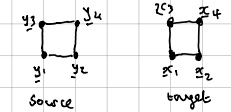
\includegraphics{setup.jpg}
\end{center}

The boxes are referred to as lying in a `surface grid', with the equivalent charges, $q_1,...,q_4$,  placed at $y_1,...y_4$. We embed the unique kernel interactions between these two boxes on a so called `convolution grid', we define them wrt to a fixed point - we can take this to be just $x_1$. These can be pre-computed and stored.

\begin{center}    
    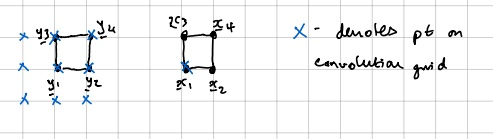
\includegraphics{conv_grid.jpg}
\end{center}

The unique interactions define the convolution grid points. We label these $K_1,...,K_9$. This is how the convolution is defined practically.

\begin{center}    
    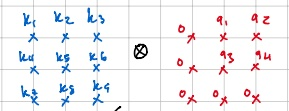
\includegraphics{conv.jpg}
\end{center}

When we go ahead and compute this, taking care to `flip' the kernel values, we find the potentials we're looking for embedded in at the following corresponding points on the convolution grid (flipped wrt to the positions of the equivalent densities). Only the four positions that correspond to the positions of the original equivalent densities are significant, the remainder can be ignored.


\begin{center}    
    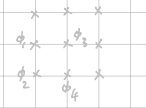
\includegraphics{result.jpg}
\end{center}


We can accelerate this convolution computation using the FFT as normal. Mathematically, this can be expressed as follows \dots


\subsection{$N$-Dimensional DFT}

The DFT takes a sequence of complex numbers $u_0, u_1, ..., u_{N-1}$ and transforms them into another sequence of complex numbers $\hat{u}_0, \hat{u}_1,...,0\hat{u}_{N-1}$, the forward and backwatf transfroms is defined as,

\begin{flalign}
    \hat{u}_k = \frac{1}{N}\sum_{j=0}^{N-1}u_j e^{-ikx_j}, \> \> k=0,1,...,N-1 \\
    u_k = \frac{1}{N}\sum_{j=0}^{N-1}\hat{u}_j e^{ikx_j}, \> \> k=0,1,...,N-1
\end{flalign}

where $x_j = 2\pi j / N$. If instead the data is arranged in a multidimensional array, $u_{j_0, j_1, ..., j_{d-1}}$ where there are $d$ index sets $j_m = 0, 1, ..., N_{m-1}$, $m \in 0, 1, ..., d-1$ with $N_m = \|j_m\|$ being the length of $j_m$. A forward $d$-dimensional DFT of the $d$-dimensional array will be computed as,

\begin{flalign}
    \hat{u}_{k_0, k_1, ..., k_{d-1}} = \sum_{j_0 = 0}^{N_0 - 1} 
    \left( \frac{\omega_0^{k_0 j_0}}{N_0} \sum_{j_1 = 0}^{N_1-1} \left(  \frac{\omega_1^{k_1j_1}}{N_1} ... \sum_{j_d-1}^{N_{d-1}-1} \frac{\omega_{d-1}^{k_{d-1}j_{d-1}}}{N_{d-1}} u_{j_0, j_1,...,j_{d-1}} \right) \right)
\end{flalign}

where $w_j = e^{\frac{-2\pi i}{N_j}}$


Normalisation in this context refers to the scaling of the output to be independent of input size. That is if you double the size of your input, e.g. via padding, the amplitude of the output frequencies should not change. This is done by dividing the output of the FFT by the length of the input array (or its square root depending on convention).

\subsection{Taking Advantage of Modern CPU Architectures}

We want to batch together computations sibling interactions and take advantage of SIMD to maximally take advantage of the cache hierarchies in modern CPUs. One strategy is as follows, we conclude by contrasting it with the BLAS3/SVD approach, and include some numerical benchmarks to contrast the two ...


    
\printbibliography[heading=bibintoc]

\end{document}
